\documentclass[border=10pt]{standalone}
%%%<
\usepackage{verbatim}
%%%>
\usepackage{pgfplots}
\pgfplotsset{width=7cm,compat=1.8}
\usepgfplotslibrary{ternary}
\begin{comment}
:Title: A ternary diagram
:Tags: 2D;Ternary diagrams;Manual
:Author: Christian Feuersänger
:Slug: ternary-diagram

The ternary library allows to draw ternary diagrams.
A ternary diagram visualizes three-component systems such that
the sum of them yields 100 percent. Ternary
diagrams are triangular axes.

This example is a (crude) copy of an example of
http://www.sv.vt.edu/classes/MSE2094_NoteBook/96ClassProj/experimental/ternary2.html
and uses area style to change cycle list and the legend appearance.

The code is from the PGFPlots 1.10 manual: "5.12 Ternary Diagrams".
\end{comment}
\begin{document}
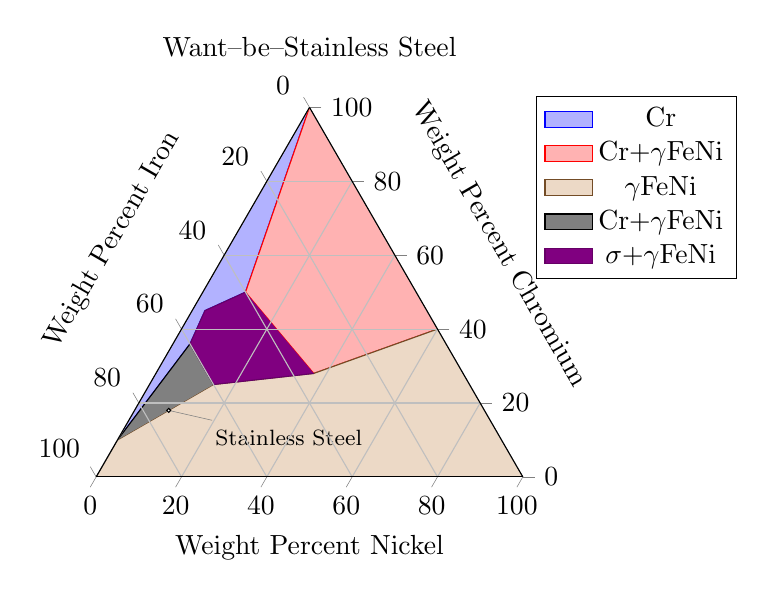
\begin{tikzpicture}
\begin{ternaryaxis}[
	title=Want--be--Stainless Steel,
	xlabel=Weight Percent Chromium,
	ylabel=Weight Percent Iron,
	zlabel=Weight Percent Nickel,
	label style=sloped,
	area style,
]
	\addplot3 table {
	A B C
	1 0 0
	0.5 0.4 0.1
	0.45 0.52 0.03
	0.36 0.6 0.04
	0.1 0.9 0
	};
	\addlegendentry{Cr}

	\addplot3 table {
	A B C
	1 0 0
	0.5 0.4 0.1
	0.28 0.35 0.37
	0.4 0 0.6
	};
	\addlegendentry{Cr+$\gamma$FeNi}

	\addplot3 table {
	0.4 0 0.6
	0.28 0.35 0.37
	0.25 0.6 0.15
	0.1 0.9 0
	0 1 0
	0 0 1
	};
	\addlegendentry{$\gamma$FeNi}

	\addplot3 table {
	0.1 0.9 0
	0.36 0.6 0.04
	0.25 0.6 0.15
	};
	\addlegendentry{Cr+$\gamma$FeNi}

	\addplot3 table {
	0.5 0.4 0.1
	0.45 0.52 0.03
	0.36 0.6 0.04
	0.25 0.6 0.15
	0.28 0.35 0.37
	};
	\addlegendentry{$\sigma$+$\gamma$FeNi}

	\node[inner sep=0.5pt,circle,draw,fill=white,
	  pin=-15:\footnotesize Stainless Steel] at (axis cs:0.18,0.74,0.08) {};
	
\end{ternaryaxis}
\end{tikzpicture}
\end{document}
